
\begin{quotation}
	The simplest quantum mechanical system, and the system which we will be most concerned with, is the \emph{qubit}. A qubit has a two-dimensional state space. [...] 
	The way a qubit differs from a bit is that superpositions of these two states, of the form $a\ket{0} + b\ket{1}$, can also exist, in which it is not possible to say that the qubit is definitely in the state $\ket0$, or definitely in the state $\ket1$.
	\cite{NC10}
\end{quotation}

\large{\textbf{The three postulates}}\footcite{NC10}
	\begin{quote}
		\textbf{Postulate 1}: Associated to any isolated physical system is a complex vector space with inner product (that is, a Hilbert space) known as the \emph{state space} of the system. 
		The system is completely described by its \emph{state vector}, which is a unit vector in the system's state space. 
	\end{quote}
	
	\begin{quote}
		\textbf{Postulate 2}: The evolution of a \emph{closed} quantum system is described by a \emph{unitary transformation}. That is, the state $\ket{\psi}$ of the system at time $t_1$ is related to the state $\ket{\psi'}$ of the system at time $t_2$ by a unitary operator $U$ which depends only on times $t_1$ and $t_2$,
		$$ \ket{\psi'} = U\ket{\psi} $$
	\end{quote}
	
	\begin{quote}
		\textbf{Postulate 3}: Quantum measurements are described by a collection $\{M_m\}$ of \emph{measurements operators}. 
		These are operators acting on the state space of the system being measured. 
		The index $m$ refers to the measurement outcomes that may occur in the experiment. If the state of the quantum system is $\ket{\psi}$ immediately before the measurement then the probability that result $m$ occur is given by 
		$$ p(m) = \bra{\psi}M_m^{\dagger}M_m\ket{\psi} \: ,$$
		and the state of the system after the measurement is 
		$$ \frac{M_m\ket{\psi}}{\sqrt{\bra{\psi}M_m^{\dagger}M_m\ket{\psi}}} \: . $$
		The measurement operators satisfy the \emph{completeness equation},
		$$\sum_m  M_m^{\dagger}M_m = I \: .$$
		The completeness equation expresses the fact that probabilities sum to one:
		$$ 1 = \sum_m p(m) = \sum_m  \bra{\psi}M_m^{\dagger}M_m\ket{\psi} \: .$$ 
	\end{quote}
	
	Quantum mechanics is a very large and complex theory. For our purposes it is enough for us to only consider the quantum system called \emph{qubit} and its rules of computation following from the tensor product algebra. 

\section{Dirac's notation}
	%	\begin{figure}[h!]
%		\centering
%		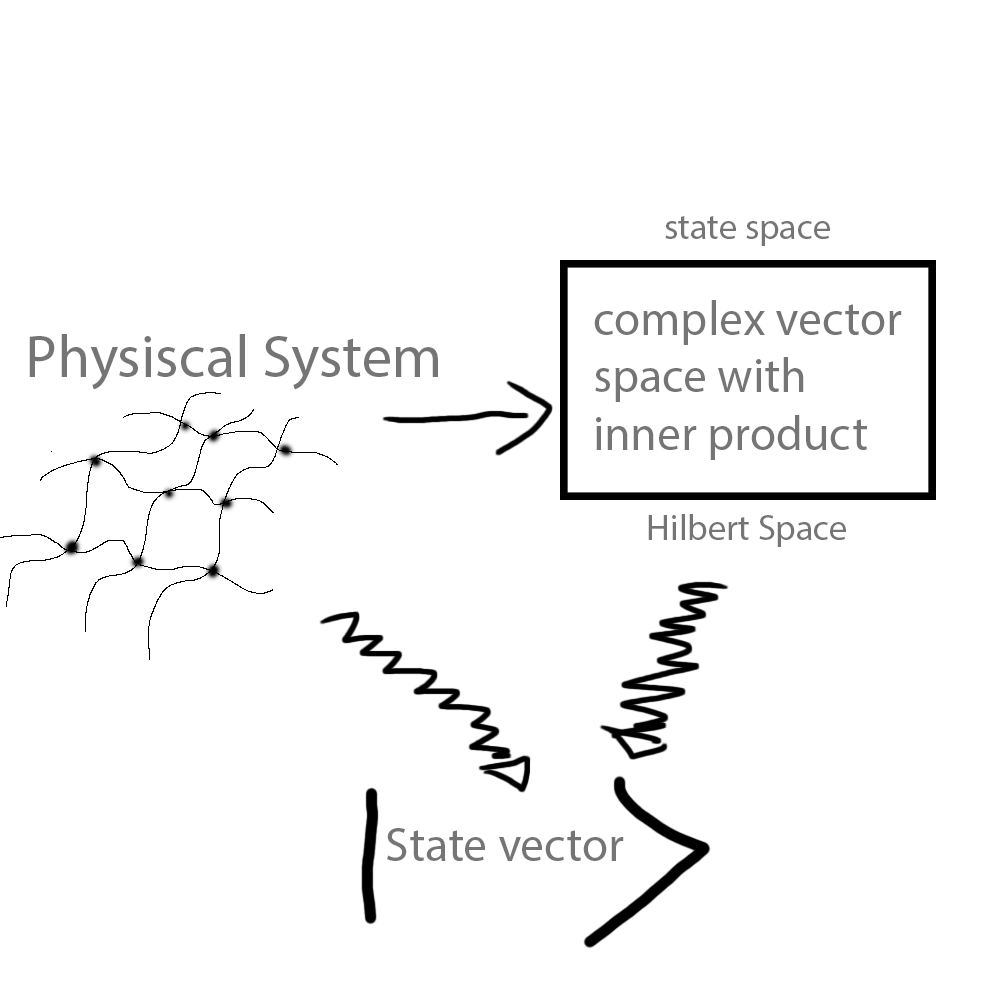
\includegraphics[scale=0.2]{images/sketch1.png} 
%		\caption{how a physical state is represented}
%	\end{figure}
	Every pure quantum state can be represented a vector in a vector space with inner product, i.e. a \emph{Hilbert space}. 
	The implication of this will be explained in the next section; for now we only look of this vector representation.\\
	 A complex Hilbert space $\H$ of dimension $n$ is isomorphic to $ \mathbb{C}^n $ with the standard inner product. 
	 In $\mathbb{C}^n $ one can choose a basis and then represent vectors with coordinates with respect to this basis.\\
	The bra-ket notation is a handy notation introduced by physicist Paul Dirac to deal with such vector representation of quantum states. 
	First of all we note that a state $\varphi '\in\H$ corresponds via the isomorphism to $ \varphi  \in \mathbb{C}^n $. It can be represented as a vector with respect of some basis as follows
	$$\ket{\varphi} = \begin{pmatrix} \varphi_1 \\ \varphi_2 \\ \vdots \end{pmatrix}	  \text{  is a coloumn "ket" vector over } \H $$
	$$\bra{\varphi}  = \begin{pmatrix} \varphi_1 & \varphi_2 & \hdots \end{pmatrix} \text{  is a row "bra" vector over } \H $$
	To be representative of a quantum state the vector has to have unitary length, $\|\varphi\|= 1$.
	Furthermore the conjugate transpose of a \emph{bra} vector is the corresponding \emph{ket} vector, and vice versa.
	$$ \bra{\varphi}^{\dagger} = \ket{\varphi} \text{,    } \ket{\varphi}^{\dagger} = \bra{\varphi}$$
	More specifically, for a complex vector space as $\H$, the components of $\bra{\varphi}$ are each the complex conjugate of the components of $\ket{\varphi}$.\\
	It is worth noting that in quantum information we will consider only vectors of finite dimensions, and more often than not, the standard basis for qubits represented by
	$$\ket0 =  \begin{pmatrix} 1 \\ 0 \end{pmatrix}
	\text{ and }
	\ket1 =  \begin{pmatrix} 0 \\ 1 \end{pmatrix}$$
	which are recognizable as the equivalent of $\vec{e_1}$ and $\vec{e_2}$ in $\mathbb{C}^2$.\\
	
	To summarize then, $\ket{\varphi}$ represents a column vector on a complex vector space with inner product equivalent to $\mathbb{C}^n$ in some basis, and $\bra{\varphi}$ is its complex conjugate.
	
	
	So if we define the matrix\footnote{The fact that the result of  $ \ketbra{w}{v} $ is indeed a matrix can be seen more directly if we remember that this is nothing less than a column-row vectors multiplication.} $A =  \ketbra{w}{v} $ we observe that
	$$ \ket{w}\braket{v}{v'} = \braket{v}{v'}\ket{w} $$	
	which is a convenient way of visualizing the action of matrix $A$. In particular if we divide it like $(\ketbra{w}{v}) (\ket{v'}) $ it is easy to interpret it as \textit{matrix $A$ acting on vector $\ket{v'}$}; but the other equivalent form $(\braket{v}{v'})(\ket{w})$ can also be seen as multiplying vector $\ket{w}$ by a value $\braket{v}{v'}$. \\
	%this part may be too similar to book, page 67...
	The meaning of this is that $\ketbra{w}{v}$ can indeed be defined as a (linear) operator from the vector space of $\ket{v}$ and $\ket{v'}$ to the vector space of $\ket{w}$. This comes in very handy when we later use it to define operations and measurements on quantum states.\\
\section{Measurements on a  basis}
    
	\subsubsection*{Linear operators}
	A linear operator between two vector spaces is defined as 
	$$ \mathbf{A}: V\longrightarrow W \text{  ,  }\ket{v_i}\mapsto A\ket{v_i}$$
	$$ \text{ linear in all inputs, i.e.  }  A\left( \sum_i a_i\ket{v_i}\right) = \sum_i a_i A\ket{v_i} \text{  for all } i $$ 
	Looking back at the definition of the matrix $ A = \ketbra{w}{v}$ we can now refer to it as a linear operator from now on. \\
	Some well-known linear operators acting on single qubits that we will use later on are the \textit{Pauli Matrices}
	$$ I = \begin{bmatrix} 1 & 0 \\ 0 & 1 \end{bmatrix}	 \quad   X = \begin{bmatrix} 0 & 1 \\ 1 & 0 \end{bmatrix}$$
	$$ Y= \begin{bmatrix} 0 & -i \\ i & 0 \end{bmatrix}	 \quad   Z = \begin{bmatrix} 1 & 0 \\ 0 & -1 \end{bmatrix}$$
	
	In particular it is safe to say that, unless stated otherwise, the operators that will be presented all have a set of properties and are called Hermitian operators, or self-adjoint operators.\\
	$$ A = A^{\dagger} \quad \Longrightarrow (A\ket{v})^{\dagger} = \bra{v}A^{\dagger} $$ 
	Operators have also to be positive, this means that it holds, for every $\ket{v}$ : $\bra{v}A\ket{v}$ is real non-negative. Any positive operator is also self-adjoint and therefore it has diagonal (spectral) representation $\sum_i \lambda_i \proj{i}$ with non-negative eigenvalues $\lambda_i$.\\    
    
\section{Quantum entanglement}

	\begin{quotation}
		There exist vectors in $V\otimes W$ that can not be represented by a single tensor product:
		Given $v_1,v_2\in V \; w_1,w_2\in W$ linear independent:
    \begin{equation*}
		v_1\otimes w_1 + v_2\otimes w_2 = v_1w_1 + v_2w_2 \in V\otimes W
    \end{equation*}
    is \emph{not} separable.
		this may be strange because on physical level tensor product is combination(merging) of quantum systems
		\end{quotation}
		\cite{Han13}